\section*{Введение}
\addcontentsline{toc}{section}{Введение}

% На данный момент в программных системах самым распространенным представлением информации, которая создается пользователем или демонстрируется ему, является текстовое представление. Оно удобно по многим причинам, но у него есть существенный недостаток - часто без дополнительного стилизирования текстовая информация слишком тяжело воспринимается. При отображении данных для пользователя необходимо явственным образом сохранять изначальную структуру информации. В большинстве случаев такое стилизирование сводится к форматированию текста, то есть добавлению или удалению не несущих информацию символов, другому преобразованию текста без изменения его семантики. Данное преобразование называется \emph{pretty printing}.

С появлением первых языков программирования особую важность приобрели языковые процессоры. \emph{Языковой процессор} (\emph{ЯП}) --- это программное средство, принимающее на вход программу в виде текста на некотором языке (программирования, разметки и т. д.) и решающее определенную задачу над этой программой. К языковым процессорам можно отнести: компиляторы, суперкомпиляторы, интерпретаторы, средства статического анализа кода, декомпиляторы, средства рефакторинга, средства реинжиниринга, интегрированные среды разработки (IDE) и др.

Первым этапом работы ЯП является \emph{синтаксический анализ}, то есть сопоставление входного текста (линейной последовательности лексем) с формальной грамматикой языка. В результате работы синтаксического анализатора ЯП получает древовидное представление программы, над которым потом происходит основная работа.

Достаточно часто возникает задача показать пользователю промежуточный или конечный результат обработки кода.
Следовательно, необходимо вернуться к текстовому представлению программы, то есть провести процедуру, обратную синтаксическому анализу. Такая задача называется \emph{pretty printing}, а соответствующий инструмент --- \emph{pretty printer}. Далее этот инструмент мы будем называть \emph{принтером}.

Одной из проблем, возникающей при разработке принтера, является то, что критерии качества его работы трудно формализуемы.
Очевидно, что одного соответствия с точки зрения синтаксиса и семантики полученного кода и древовидного представления недостаточно. Рассмотрим программы на рисунках~\ref{fig:wikiExUnfor} и \ref{fig:wikiExBSD}.

\begin{figure}[h!]
	\centering
	% \inputminted{c}{codes/wikiExUnfor.c}
	\lstinputlisting[language=C]{Podkopaev/codes/wikiExUnfor.c}
	\caption{Неформатированный код}
	\label{fig:wikiExUnfor}
\end{figure}

\begin{figure}[h!]
	\centering
	% \inputminted{c}{codes/wikiExBSD.c}
	\lstinputlisting[language=C]{Podkopaev/codes/wikiExBSD.c}
	\caption{Форматированный код}
	\label{fig:wikiExBSD}
\end{figure}

Они эквиваленты синтаксически и семантически с точки зрения компилятора C, но для пользователя вариант с рисунка~\ref{fig:wikiExBSD} предпочтительней, так как он проще для восприятия. Как мы видим, при отображении данных необходимо явным для пользователя образом представлять иерархическую структуру информации. В большинстве случаев решение этой задачи сводится к добавлению или удалению символов, не несущих информации для синтаксического анализа, или другому преобразованию текста без изменения его семантики.

Кроме того определенную сложность в описание и исполнение конкретного принтера вносит тот факт, что в большинстве случаев нельзя однозначным образом сопоставить синтаксическую конструкцию с единственным представлением. Необходима вариативность в зависимости от дополнительных условий, наложенных на результат его работы.

Рассмотрим небольшой пример. Пользователь задает условие вида: ``последовательные операторы пишутся на одной строке, если помещаются в $N$ символов, а иначе --- на разных строках''.

\begin{figure}[h!]
	\centering
	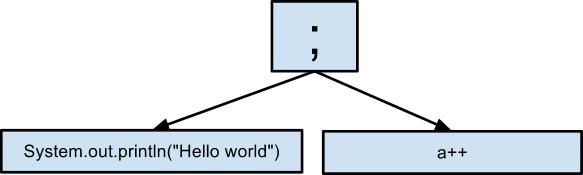
\includegraphics[width=0.8\textwidth]{seqTree}
	\caption{Последовательные операторы}
	\label{fig:seqImage}
\end{figure}

На рисунке~\ref{fig:seqImage} изображено синтаксическое дерево последовательности двух операторов. Такое дерево, согласно заданному правилу, может быть напечатано одним из двух вариантов (рисунки~\ref{fig:seqCode1}, ~\ref{fig:seqCode2}).

\begin{figure}[h!]
	\centering
	% \inputminted{c}{codes/seqCode1.java}
	\lstinputlisting[language=Java]{Podkopaev/codes/seqCode1.java}
	\caption{Последовательные операторы в строчку}
	\label{fig:seqCode1}
\end{figure}

\begin{figure}[h!]
	\centering
	% \inputminted{c}{codes/seqCode2.java}
	\lstinputlisting[language=Java]{Podkopaev/codes/seqCode2.java}
	\caption{Последовательные операторы в несколько строк}
	\label{fig:seqCode2}
\end{figure}

Выбор происходит в зависимости от ширины вывода. Так, при ширине равной 35 символов (длина строки <<System.out.println(“Hello world”); >>), должен выбираться вариант, изображенный на рисунке~\ref{fig:seqCode2}, так как код на рисунке~\ref{fig:seqCode1} имеет ширину более 35 символов.
Могут быть заданы и более сложные условия.

Рассмотрим другой пример. Пусть нам нужно текстовое представление синтаксического дерева конструкции “\lstinline{if}”, и заданы шаблоны c рисунков~\ref{fig:ifTemplate2} и \ref{fig:ifTemplate1}, причем вариант, изображенный на рисунке~\ref{fig:ifTemplate2} выбирается в случае, если условие и ветки могут быть напечатаны в одну строчку.

\begin{figure}[h!]
	\subfloat[]{
		\lstinputlisting[language=Haskell]{Podkopaev/codes/ifTemplate2.hs}
		\label{fig:ifTemplate2}	
	}
	\quad
	\subfloat[]{
		\lstinputlisting[language=Haskell]{Podkopaev/codes/ifTemplate1.hs}
		\label{fig:ifTemplate1}	
	}
	\caption{Представления для конструкции “\lstinline{if}”}
\end{figure}


Тогда для деревьев, представленных на рисунках \ref{fig:ifImage1} и \ref{fig:ifImage2}, будут напечатаны коды с рисунков \ref{fig:ifCode1} и \ref{fig:ifCode2} соответственно.

\begin{figure}[h!]
	\subfloat[]{
		\centering
		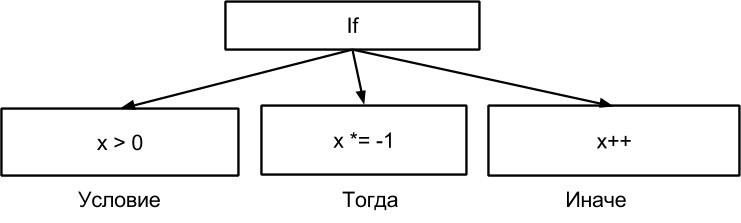
\includegraphics[width=0.6\textwidth]{if1}
		\label{fig:ifImage1}
	}
	\quad
	\subfloat[]{
		\centering
		% \inputminted{haskell}{codes/ifCode1.hs}
		\lstinputlisting[language=Haskell]{Podkopaev/codes/ifCode1.hs}
		\label{fig:ifCode1}	
	}

	\caption{Использование представления с рис.~\ref{fig:ifTemplate2}}
\end{figure}

\begin{figure}[h!]
	\subfloat[]{
		\centering
		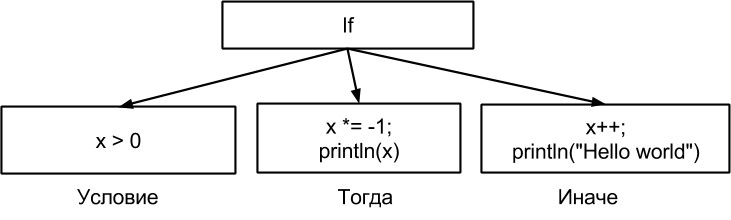
\includegraphics[width=.55\textwidth]{if2}
		\label{fig:ifImage2}	
	}
	\quad
	\subfloat[]{
		\centering
		% \inputminted{haskell}{codes/ifCode2.hs}
		\lstinputlisting[language=Haskell]{Podkopaev/codes/ifCode2.hs}
		\label{fig:ifCode2}	
	}

	\caption{Использование представления с рис.~\ref{fig:ifTemplate1}}
\end{figure}

% Постановка задачи
То, что не существует четких критериев красоты кода, а также отсутствие библиотек, предоставляющих возможность описать принтер в виде, подобном
рассмотренному примеру с конструкцией “\lstinline{if}”, то есть с помощью шаблонов, часто приводит к тому, что принтеры становятся крайне сложными и наполненными эвристиками.

Задачей данной работы было изучение существующих подходов к построению принтеров в рамках функциональных языков программирования и разработка способа определения принтеров с помощью синтаксических шаблонов.
